
\documentclass[letterpaper,hide notes,xcolor={table,svgnames},pdftex]{beamer}
\def\showexamples{t}


%\usepackage[svgnames]{xcolor}

%% Demo talk
%\documentclass[letterpaper,notes=show]{beamer}

\usecolortheme{crane}%seahorse crane
\setbeamertemplate{navigation symbols}{}

\usetheme{MyPittsburgh}
%\usetheme{Frankfurt}

%\usepackage{tipa}

\usepackage{hyperref}
\usepackage{graphicx,xspace}
\usepackage[normalem]{ulem}

\newcommand\SF[1]{$\bigstar$\footnote{SF: #1}}

\usepackage{paratype}
\renewcommand*\familydefault{\sfdefault} %% Only if the base font of the document is to be sans serif
\usepackage[zerostyle=c]{newtxtt}
\usepackage[T1]{fontenc}

\newcounter{tmpnumSlide}
\newcounter{tmpnumNote}

\usepackage{xcolor}
\usepackage{tabu}
\definecolor{light-gray}{gray}{0.75}
\taburulecolor{light-gray}

% old question code
%\newcommand\question[1]{{$\bigstar$ \small \onlySlide{2}{#1}}}
% \newcommand\nquestion[1]{\ifdefined \presentationonly \textcircled{?} \fi \note{\par{\Large \textbf{?}} #1}}
% \newcommand\nanswer[1]{\note{\par{\Large \textbf{A}} #1}}


 \newcommand\mnote[1]{%
   \addtocounter{tmpnumSlide}{1}
   \ifdefined\showcues {~\tiny\fbox{\arabic{tmpnumSlide}}}\fi
   \note{\setlength{\parskip}{1ex}\addtocounter{tmpnumNote}{1}\textbf{\Large \arabic{tmpnumNote}:} {#1\par}}}

\newcommand\mmnote[1]{\note{\setlength{\parskip}{1ex}#1\par}}

%\newcommand\mnote[2][]{\ifdefined\handoutwithnotes {~\tiny\fbox{#1}}\fi
% \note{\setlength{\parskip}{1ex}\textbf{\Large #1:} #2\par}}

%\newcommand\mnote[2][]{{\tiny\fbox{#1}} \note{\setlength{\parskip}{1ex}\textbf{\Large #1:} #2\par}}

\newcommand\mquestion[2]{{~\color{red}\fbox{?}}\note{\setlength{\parskip}{1ex}\par{\Large \textbf{?}} #1} \note{\setlength{\parskip}{1ex}\par{\Large \textbf{A}} #2\par}\ifdefined \presentationonly \pause \fi}

\newcommand\blackboard[1]{%
\ifdefined   \showblackboard
  {#1}
  \else {\begin{center} \fbox{\colorbox{blue!30}{%
         \begin{minipage}{.95\linewidth}%
           \hspace{\stretch{1}} Some space intentionally left blank; done at the blackboard.%
         \end{minipage}}}\end{center}}%
         \fi%
}



%\newcommand\q{\tikz \node[thick,color=black,shape=circle]{?};}
%\newcommand\q{\ifdefined \presentationonly \textcircled{?} \fi}

\usepackage{listings}
\lstset{%
  keywordstyle=\bfseries,
  aboveskip=15pt,
  belowskip=15pt,
  captionpos=b,
  identifierstyle=\ttfamily,
  escapeinside={(*@}{@*)},
  stringstyle=\ttfamiliy,
  frame=lines,
  numbers=left, basicstyle=\scriptsize, numberstyle=\tiny, stepnumber=0, numbersep=2pt}

\usepackage{siunitx}
\newcommand\sius[1]{\num[group-separator = {,}]{#1}\si{\micro\second}}
\newcommand\sims[1]{\num[group-separator = {,}]{#1}\si{\milli\second}}
\newcommand\sins[1]{\num[group-separator = {,}]{#1}\si{\nano\second}}
\sisetup{group-separator = {,}, group-digits = true}

%% -------------------- tikz --------------------
\usepackage{tikz}
\usetikzlibrary{positioning}
\usetikzlibrary{arrows,backgrounds,automata,decorations.shapes,decorations.pathmorphing,decorations.markings,decorations.text}

\tikzstyle{place}=[circle,draw=blue!50,fill=blue!20,thick, inner sep=0pt,minimum size=6mm]
\tikzstyle{transition}=[rectangle,draw=black!50,fill=black!20,thick, inner sep=0pt,minimum size=4mm]

\tikzstyle{block}=[rectangle,draw=black, thick, inner sep=5pt]
\tikzstyle{bullet}=[circle,draw=black, fill=black, thin, inner sep=2pt]

\tikzstyle{pre}=[<-,shorten <=1pt,>=stealth',semithick]
\tikzstyle{post}=[->,shorten >=1pt,>=stealth',semithick]
\tikzstyle{bi}=[<->,shorten >=1pt,shorten <=1pt, >=stealth',semithick]

\tikzstyle{mut}=[-,>=stealth',semithick]

\tikzstyle{treereset}=[dashed,->, shorten >=1pt,>=stealth',thin]

\usepackage{ifmtarg}
\usepackage{xifthen}
\makeatletter
% new counter to now which frame it is within the sequence
\newcounter{multiframecounter}
% initialize buffer for previously used frame title
\gdef\lastframetitle{\textit{undefined}}
% new environment for a multi-frame
\newenvironment{multiframe}[1][]{%
\ifthenelse{\isempty{#1}}{%
% if no frame title was set via optional parameter,
% only increase sequence counter by 1
\addtocounter{multiframecounter}{1}%
}{%
% new frame title has been provided, thus
% reset sequence counter to 1 and buffer frame title for later use
\setcounter{multiframecounter}{1}%
\gdef\lastframetitle{#1}%
}%
% start conventional frame environment and
% automatically set frame title followed by sequence counter
\begin{frame}%
\frametitle{\lastframetitle~{\normalfont(\arabic{multiframecounter})}}%
}{%
\end{frame}%
}
\makeatother

\makeatletter
\newdimen\tu@tmpa%
\newdimen\ydiffl%
\newdimen\xdiffl%
\newcommand\ydiff[2]{%
    \coordinate (tmpnamea) at (#1);%
    \coordinate (tmpnameb) at (#2);%
    \pgfextracty{\tu@tmpa}{\pgfpointanchor{tmpnamea}{center}}%
    \pgfextracty{\ydiffl}{\pgfpointanchor{tmpnameb}{center}}%
    \advance\ydiffl by -\tu@tmpa%
}
\newcommand\xdiff[2]{%
    \coordinate (tmpnamea) at (#1);%
    \coordinate (tmpnameb) at (#2);%
    \pgfextractx{\tu@tmpa}{\pgfpointanchor{tmpnamea}{center}}%
    \pgfextractx{\xdiffl}{\pgfpointanchor{tmpnameb}{center}}%
    \advance\xdiffl by -\tu@tmpa%
}
\makeatother
\newcommand{\copyrightbox}[3][r]{%
\begin{tikzpicture}%
\node[inner sep=0pt,minimum size=2em](ciimage){#2};
\usefont{OT1}{phv}{n}{n}\fontsize{4}{4}\selectfont
\ydiff{ciimage.south}{ciimage.north}
\xdiff{ciimage.west}{ciimage.east}
\ifthenelse{\equal{#1}{r}}{%
\node[inner sep=0pt,right=1ex of ciimage.south east,anchor=north west,rotate=90]%
{\raggedleft\color{black!50}\parbox{\the\ydiffl}{\raggedright{}#3}};%
}{%
\ifthenelse{\equal{#1}{l}}{%
\node[inner sep=0pt,right=1ex of ciimage.south west,anchor=south west,rotate=90]%
{\raggedleft\color{black!50}\parbox{\the\ydiffl}{\raggedright{}#3}};%
}{%
\node[inner sep=0pt,below=1ex of ciimage.south west,anchor=north west]%
{\raggedleft\color{black!50}\parbox{\the\xdiffl}{\raggedright{}#3}};%
}
}
\end{tikzpicture}
}


%% --------------------

%\usepackage[excludeor]{everyhook}
%\PushPreHook{par}{\setbox0=\lastbox\llap{MUH}}\box0}

%\vspace*{\stretch{1}

%\setbox0=\lastbox \llap{\textbullet\enskip}\box0}

\setlength{\parskip}{\fill}

\newcommand\noskips{\setlength{\parskip}{1ex}}
\newcommand\doskips{\setlength{\parskip}{\fill}}

\newcommand\xx{\par\vspace*{\stretch{1}}\par}
\newcommand\xxs{\par\vspace*{2ex}\par}
\newcommand\tuple[1]{\langle #1 \rangle}
\newcommand\code[1]{{\sf \footnotesize #1}}
\newcommand\ex[1]{\uline{Example:} \ifdefined \presentationonly \pause \fi
  \ifdefined\showexamples#1\xspace\else{\uline{\hspace*{2cm}}}\fi}

\newcommand\ceil[1]{\lceil #1 \rceil}


\AtBeginSection[]
{
   \begin{frame}
       \frametitle{Outline}
       \tableofcontents[currentsection]
   \end{frame}
}



\pgfdeclarelayer{edgelayer}
\pgfdeclarelayer{nodelayer}
\pgfsetlayers{edgelayer,nodelayer,main}

\tikzstyle{none}=[inner sep=0pt]
\tikzstyle{rn}=[circle,fill=Red,draw=Black,line width=0.8 pt]
\tikzstyle{gn}=[circle,fill=Lime,draw=Black,line width=0.8 pt]
\tikzstyle{yn}=[circle,fill=Yellow,draw=Black,line width=0.8 pt]
\tikzstyle{empty}=[circle,fill=White,draw=Black]
\tikzstyle{bw} = [rectangle, draw, fill=blue!20, 
    text width=4em, text centered, rounded corners, minimum height=2em]
    
    \newcommand{\CcNote}[1]{% longname
	This work is licensed under the \textit{Creative Commons #1 3.0 License}.%
}
\newcommand{\CcImageBy}[1]{%
	\includegraphics[scale=#1]{creative_commons/cc_by_30.pdf}%
}
\newcommand{\CcImageSa}[1]{%
	\includegraphics[scale=#1]{creative_commons/cc_sa_30.pdf}%
}
\newcommand{\CcImageNc}[1]{%
	\includegraphics[scale=#1]{creative_commons/cc_nc_30.pdf}%
}
\newcommand{\CcGroupBySa}[2]{% zoom, gap
	\CcImageBy{#1}\hspace*{#2}\CcImageNc{#1}\hspace*{#2}\CcImageSa{#1}%
}
\newcommand{\CcLongnameByNcSa}{Attribution-NonCommercial-ShareAlike}


\newenvironment{changemargin}[1]{% 
  \begin{list}{}{% 
    \setlength{\topsep}{0pt}% 
    \setlength{\leftmargin}{#1}% 
    \setlength{\rightmargin}{1em}
    \setlength{\listparindent}{\parindent}% 
    \setlength{\itemindent}{\parindent}% 
    \setlength{\parsep}{\parskip}% 
  }% 
  \item[]}{\end{list}} 




\title{Lecture 25 --- Memory Management }

\author{J. Zarnett\\
\texttt{jzarnett@uwaterloo.ca}}
\institute{Department of Electrical and Computer Engineering \\
  University of Waterloo}
\date{\today}

\begin{document}

\begin{frame}
  \titlepage
  
  \begin{center}
  \small{Acknowledgments: W.D. Bishop}
  \end{center}
\end{frame}

\begin{frame}
\frametitle{Stack and Heap}
We often talk of storing a variable in memory, but this glosses over how exactly memory works, and this is a non-trivial topic.

A program has two areas of memory: the \alert{stack} and \alert{heap}.

Both are simply designated areas of memory related to the running program, but they are modelled and used in different ways.

\end{frame}

\begin{frame}
\frametitle{Stack vs. Heap: Visually}

\begin{center}
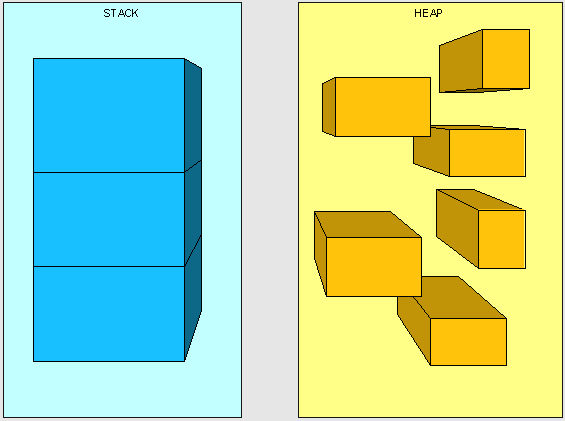
\includegraphics[width=0.75\textwidth]{images/stackheap.png}\\
{\tiny Source: \url{http://www.c-sharpcorner.com/UploadFile/rmcochran/csharp_memory01122006130034PM/csharp_memory.aspx?ArticleID=9adb0e3c-b3f6-40b5-98b5-413b6d348b91} }
\end{center}

\end{frame}

\begin{frame}
\frametitle{The Stack}

The stack keeps track of what is executing in our code.

Imagine the stack as a series of boxes stacked one on top of another.

Every time we call a function, we put another box on the pile.

This box, actually called a \alert{frame}, contains the parameters, local variables, and the return value of the function.

We can only access the box currently on top of the pile.

\end{frame}

\begin{frame}
\frametitle{The Stack}

Value types (like \texttt{int}, \texttt{double}, and \texttt{struct}) are allocated on the stack.

Imagine we are in a method \texttt{method1()}.

A statement like \texttt{int i = 4;} allocates the variable \texttt{i} on the stack.\\
\quad It is of \texttt{int} size and appears on the top of the stack.\\
\quad It is then available within \texttt{method1}. 

If the next statement is \texttt{int j = 0;} then another variable is allocated at the address immediately above the location for \texttt{i}.

These variables exist only as long as \texttt{method1()} is running.

\end{frame}

\begin{frame}
\frametitle{The Stack}
When a function returns (finishes execution), the box on top of the stack is thrown away and we can use the stuff in the box below.

Thus, stack data is discarded aggressively (i.e., as soon as possible).

You will learn more about how the stack works and is structured in ECE~254 (Operating Systems).

\end{frame}

\begin{frame}
\frametitle{Method Return}

\begin{center}
	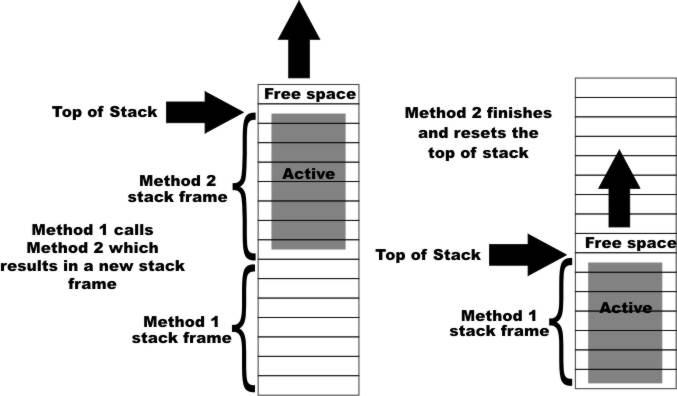
\includegraphics[width=\textwidth]{images/stackframes.jpg}
\end{center}
Source: \url{http://www.i-programmer.info/ebooks/deep-c/363}
\end{frame}


\begin{frame}
\frametitle{More about the Stack}

Stack space is limited in practice. Recall that recursion can result in a Stack Overflow error: this is what happens when we run out of space.

This was the result of infinite recursion: calling the function too many times (stacking too many boxes).

In normal operations, however, we will not run out of stack space.

But what if we allocate a reference type...?

\end{frame}

\begin{frame}
\frametitle{The Heap}

Reference types are allocated on the heap.

If a reference type is allocated (the \texttt{new} keyword is used), the object instantiated is allocated on the heap.

This applies also to strings, arrays, and other classes.

The internals of the heap are beyond the scope of the course.\\
\quad But you will examine it later in ECE~250.

\end{frame}

\begin{frame}
\frametitle{Discarding Objects in the Heap}

We saw we don't have to de-allocate a variable allocated on the stack.\\
\quad The end of the function takes care of that for us.

Heap objects, however, can outlive the functions that created them.

Heap space is also limited by the amount of memory available on the machine. This is typically much larger than the space for the stack. 

Still, we need a way to discard things. 

Unused objects in memory don't have any value, and they prevent other applications from using that memory.

\end{frame}

\begin{frame}
\frametitle{Garbage}

Recall from earlier the concept of variable scope.

If a reference to an object goes out of scope, that reference can no longer be used to access the object to which it refers.

If there are no valid references to an object, that object is no longer accessible and cannot be used for anything.

Such an inaccessible object is considered ``garbage''.

\end{frame}

\begin{frame}
\frametitle{Garbage Collection}

The C\# approach to cleaning up garbage is called \alert{Garbage Collection}.

Garbage objects are not discarded aggressively.\\
\quad They will be cleaned automatically by the garbage collector.\\
\quad The garbage collector runs when the system chooses.\\
\quad This may ``waste'' some memory, but can improve performance.

There is no simple way of figuring out when an object on the heap is not needed anymore, so the process of garbage collection is complex.

\end{frame}

\begin{frame}
\frametitle{Garbage Collection}

How does garbage collection work?
\begin{itemize}
\item Memory is allocated whenever an object is constructed
\item Once the scope of an object ends, the object becomes ``garbage''
\item Programmers do not indicate when an object is no longer needed
\item The memory associated with garbage objects is made available to the system when garbage collection is performed
\end{itemize}

The system decides when garbage collection is performed; the programmer does not indicate this. 

\end{frame}

\begin{frame}
\frametitle{Manual Memory Management}

In languages like C++, developers also do memory deallocation:\\
\quad The language and run-time do not implement garbage collection.\\
\quad This can easily lead to \alert{memory leaks}.

A memory leak is when some area of memory remains allocated even though it is no longer needed.

Over time, a memory leak can reduce the performance of the computer by reducing the amount of available memory. 

If available memory is exhausted, this may lead to a crash.

\end{frame}

\begin{frame}
\frametitle{Pros of Garbage Collection}
Garbage collection has numerous advantages:

\begin{itemize}
	\item Simplifies the design of complex applications
	\item Enhances code quality by eliminating memory leaks
	\item Enhances developer productivity
	\item Permits program to optimize memory utilization through compaction
\end{itemize}
\end{frame}

\begin{frame}
\frametitle{Cons of Garbage Collection}

It also has some disadvantages:
\begin{itemize}
	\item Limits developer control over the de-allocation of memory
	\item Introduces overhead to monitor when objects become garbage
	\item Runs at unpredictable times (a problem in real-time systems)
	\item Often temporarily halts the program executing while it cleans up (also a problem in real-time systems)
\end{itemize}
\end{frame}

\begin{frame}
\frametitle{Memory Management in C\#}

C\# uses references to keep track of heap allocated objects.

C\# automatically manages memory which means that reference type objects can be relocated (moved in memory) dynamically.

Objects are allocated in the first available memory address where an appropriately-sized block of memory is found.

Example: the first address may have space for an \texttt{int[]} array of capacity 10, but the request is to allocate an array of capacity 20.

\end{frame}

\begin{frame}
\frametitle{Memory Management in C\#}

Over time, some objects go out of scope and become garbage.

The garbage collector frees up memory containing garbage and it moves objects to make larger contiguous blocks of free memory.

To allocate a new object, a block of memory of the size of that object will be needed. If none is found, that object cannot be allocated.

References have a memory address associated with them.

When an object is relocated, the value is changed to indicate the new memory address of that object.

\end{frame}

\begin{frame}[fragile]
\frametitle{Heap Memory Management Example}

In the following code, three reference objects are instantiated:

\begin{verbatim}
Object a = new Object( );
Object b = new Object( );
Object c = new Object( );
\end{verbatim}

There are three references (\texttt{a, b, c}) that refer to three distinct locations in the heap.

\begin{center}
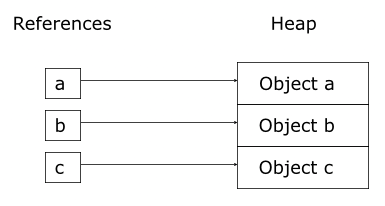
\includegraphics[width=0.5\textwidth]{images/heapABC.png}
\end{center}

\end{frame}

\begin{frame}
\frametitle{Heap Memory Management Example}

Now: \texttt{ b = null; }

\begin{center}
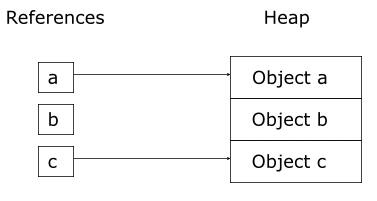
\includegraphics[width=0.5\textwidth]{images/heapAC.png}
\end{center}

Object b has gone out of scope and is no longer reachable.\\
\quad It is garbage and may be collected when the garbage collector runs.

\end{frame}

\begin{frame}
\frametitle{Heap Memory Management Example}

When garbage collection runs, Object b is no longer there; its location is now free memory.

\begin{center}
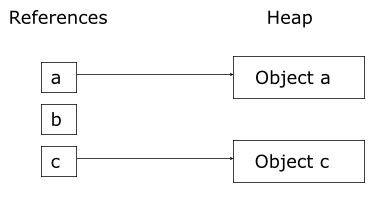
\includegraphics[width=0.5\textwidth]{images/heapNoB.png}
\end{center}

\end{frame}

\begin{frame}
\frametitle{Heap Memory Management Example}

When garbage collection runs, it may ``compact'' the objects in memory to reduce the spaces between allocated objects.

\begin{center}
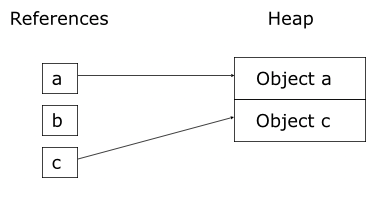
\includegraphics[width=0.5\textwidth]{images/heapCompact.png}
\end{center}

This also produces larger contiguous blocks of free memory.

\end{frame}

\begin{frame}
\frametitle{Why Compact Memory?}

Why does the garbage collection process compact memory?

To avoid the situation where there is enough available memory free in the system, but no single contiguous block to hold an allocation.

If there are two blocks that can hold  \texttt{int[]} arrays of capacity 10, we could allocate an array up to a capacity of 20 if they are combined.


\end{frame}


\end{document}

